\documentclass[type=dr, dr=rernat, accentcolor=tud7b,colorbacktitle, bigchapter, openright, twoside, 12pt ]{tudthesis}
%\documentclass[11pt,twoside,a4paper]{article}
\usepackage[english]{babel} 
\usepackage[utf8]{inputenc}
\usepackage{graphicx}
\usepackage{pstricks}
\usepackage{psfrag}
\usepackage{enumerate}
\usepackage{float}
\usepackage{epsfig}
\usepackage{geometry}
\usepackage{subfigure}
\usepackage{rotating}
\usepackage{minitoc}
%\usepackage{appendix}

%%%% 1 1/2 facher Zeilenabstand:	
\usepackage{setspace}
\onehalfspacing




\begin{document}
\chapter{Motion Management in Treatment Planning}
\label{chapter:vmm}
\minitoc

\section{Introduction}

Effects of motion can have a significant impact on a radiation treatment (see Section \textbf{ref!}). Therefore a proper investigation is necessary for each specific treatment and patient. There are several motion mitigation techniques available ranging from beam delivery, patient immobilization to treatment planning \textbf{Ref!}.

One of the steps for motion mitigation is proper and frequent imaging. While most commercial treatment planning software provide rigid registration between different images, deformable image registration (DIR) is currently rarely used. Even though it better quantifies anatomical and biological variations \textbf{Cite 1 varadhan). DIR is essential as well in photon as in ion radiotherapy, with usage in adaptive radiotherapy (2,3 vradhan), 4D optimization and dose calculation, contour propagation (1-11 wu) and in other categories besides radiotherapy as well (4-10 vardhan). Several different DIR algorithms are avaliable, such as B-spline, Deamons, linear elastic finite element, optical flow, viscous fluid (11-15 vardhan), etc.
	
One of the reasons for the lack of DIR in commercial software is due to unavailable validation methods. While several exist, none of them are definitive and most of them are time consuming. It is possible to evaluate DIR with deformable phantoms, where the type and size of deformation is known \textbf{25-27 varadhan}. However such quality assurance is time consuming and cannot be used in everyday clinical workflow. 

DIR validation can also be based on landmark positions, specifically their location before and after registration. In absence of externally planted markers, locating landmarks in patient anatomy can be time consuming and difficult to identify in low-contrast regions \textbf{cite varadhan}. Another option is to compare delineated contours with propagated ones. It is more efficient technique than landmark checks, however it is also time consuming and it also does not address region within the contour.

In this chapter tools to handle motion management, DIR and DIR validation will be presented. Tools were constructed for open-source software 3D Slicer, described in Section~\ref{Slicer}. In Section~\ref{Registration} details on DIR procedures will be explained. Next, Section~\ref{DIRQA} will address the issue of DIR validation - an extensive tool with various feature to tackle DIR validation will be presented. Section~\ref{Contour} will be about contour visualization. Last two sections in implementation part will be about a tool to display organ motion amplitude and generation of a mid-ventilation CT. Validation of DIR and DIR quality assurance will be presented in the Section~\ref{Verification}. Summary and discussion will be given last to sum up.

\section{Implementation}

\subsection{3D Slicer}
\label{Slicer}

3D Slicer (Slicer) is a software platform for analysis and visualization of medical images \cite{Slicer, Fedorov2012}. Slicer is a free, open-source software (BSD-style license) available on Windows, MacOSX and Linux operating systems. Among other, Slicer can:

\begin{itemize}
	\item Handle a vriety of image formats, including DICOM, NRRD and MHA
	\item Visualize voxel images, polygonal meshes and volume renderings
	\item Perform registration (rigid and non-rigid) and display results
	\item Automatic image segmentation
	\item Analyse and visualize diffusion tensor image data
	\item Track devices for image-guided procedures
\end{itemize}

The fundation of Slicer is written in C++ and it's functions can be accessed also with Python to provide rapid, iterative development. Graphical user interface is built in Qt. Visualization is based on VTK, a graphical library commonly used in scientific research.

Slicer is a research tool and as such offers tools to implement new functionalities in the form of 3D Slicer extensions. That can either be execution of external command-line programs, writing modules with new features or automate Slicer processes in form of scripted modules. 
In the Sections \textbf{Ref} different Slicer modules will be presented, which were all developed in the scope of this thesis. The purpose of the module is to quantify and visualize patient motion as well as provide quality assurance of the the obtained results.

\subsection{Registration}
\label{Registration}

The changes in patient anatomy can be seen on CT (4DCT) or MRI scan. To assest this changes a registration must be preformed. Registration can be made between different imaging modaleteis, scans from different days or phases in 4DCT. Different algorithms and software is avaliable
for image registration. However, the result is always a transformation map \cite{Richter2012}. 

\begin{equation}
\label{df}
x' = x + u_{ri}(x)
\end{equation} 

Here, $x$ and $x'$ are points in states $r$ and $i$, respectively and $u_{ri}$ is a vector field representation of the transformation map. $u_{ri}$ can among others be used for assesing motion amplitudes, contour propagation and 4D dose reconstruction. It is important to note
that for certain steps in 4D treatment planning require also inverse registration, from state $i$ to $r$ \cite{Richter2012}.

A comonlly used software for registration in medical research is Plastimatch \cite{Shackleford2010}. It is free and open-source software, avaliable as a command-line executable program. Plastimatch B-spline registration is also available in Slicer as an external module, SlicerRT \cite{Pinter2012}.  
The integration of Plastimatch in Slicer brings the advantage of a graphic user interface and hence a quick modification of parameters. However, the disadvantage comes when a large number of registrations is required, since a user presence is required. In a 4DCT registration
there are $2(N-1)$ registrations required - from reference phase to each of $N$ states of 4DCT and vice versa, except for the reference phase itself. Typical 4DCT consist of 10 phases, therefore a automatic registration of a 4DCT is a necessity, since each registration takes from 15-30 minutes.

Rather than just automatically loading different phases and registering them in Slicer a patient hierarchy concept was introduced and is explained in next section. After patient hierarchy is created, registration is then done from reference phase to all other phases and vice versa. 

\subsubsection{Patient hierarchy} 

Patient hierarchy followed a subject hierarchy principle in Slicer. It was desigened for a clear overview of registration process, DIRQA and all resulting files. There are several levels in patient hierarchy. Each level also has different attributes,
where details such as file path or reference phase are written.

\begin{itemize}
	\item Level 1: \textbf{Patient name} - seperates different patients.
	\item Level 2: \textbf{Registration node} - seperates between different registration, e.g. registration between 4DCT phases, between CT and 4DCT, MRI and CT... 
	\subitem The file directory of image, vector field and registration quality files is stored as an attribute. Additionally, there are number of phases to be registered and which phase is the reference one.
	\item Level 3: \textbf{Registration phase} - specific registration phase. Registration is done between all phases and the reference one. There have to be at least two phases
	\item Level 4: \textbf{Node} - can be either an image, a vector field, an inverse vector field or any of DIRQA nodes (see Section~\ref{DIRQA}).
	\subitem Exact file paths for specific node is stored as an attribute.
\end{itemize}

Patient hierarchy can be constructed in two ways. First option is to manually crate the whole patient hierarchy, from top to bottom level, with necessary attributes. Second option is using automatic script to look for files on hard drive and create corresponding levels in patient hierarchy. This
is possible only, if some conventions are used regarding file names and locations.

\subsection{Registration Quality Checks}
\label{DIRQA}

In order to provide visual and quantitative assessment of the registration quality a \textbf{Deformable Image Registration Quality Assurance} (DIRQA) module was created. It provides different image checks (false color, checkerboard, absolute difference, flicker, movie and landmark positions) and vector checks (jacobian and inverse consistency error). Details on all different checks will be explained in this section. Reference image, warped image, vector and inverse vector (vector from reference to moving phase) are used as inputs for DIRQA module. Additionaly landmarks and region of interest (ROI) can be used as an input.

\subsubsection{False color}
\label{Sec:FalseColor}

A good way to see difference between two images is to overlay them. However, since CT scans are usually displayed in grayscale color code, the differences can become indistinguishable. Especially if the images are quite similar, as reference and warped image usually are. With applying opposite color code to overlaying images two things are achieved. Firstly, regions were the registration was successful will be in grayscale. Next, the differences will be in color of image they belong to. In the module we used (?) red and green color code for reference and warped image respectively. 

\subsubsection{Checkerboard}

As the name suggests, checkerboard creates an image of tiles. Each tile alternates between reference and warped image. The differences between two images become apparent if there is no smooth transition from one tile to the next. The number of tiles can be manually selected. While the checkerboard offers clear indication of differences, it requires user to spot them - similar to false color.

\subsubsection{Absolute difference} 

To stress the difference between reference and warped image an absolute difference between voxel values is calculated and displayed. New image is generated, with voxels populated as the absolute difference between reference and warped image voxel values. Furthermore, average, standard deviation, minimum and maximum of absolute differneces are calulcated for quantitative assessment of registration quality (in ideal case all values would be 0).

The absolute difference feature is similar to false color, but it displays differences clearer and it also provides quantitative values. In contrast to false color which only relies on user examination.

To spare computational time or to focus on a specific region, absolute difference can also be calculated just on a specific ROI (if used as an input). Usually ROI around patient body is selected, rather than calculating on a whole patient CT.

\subsubsection{Movie}

Medical images are usually quite large - typical CT image consist of $512 \times 512 \times 100$ pixels, which makes inspecting image checks (false color, checkerboard, absolute difference) a time-consuming task. Movie feature allows for smoother display of different image slices. User selects, which view he would like to inspect (axial, sagital or coronal) and presses start. Selected views then start scrolling from one limit to the other. It allows user to focus on registration details, rather than scrolling through slices.

Movie and flicker (explained below) do not offer any specific registration check, but improve the process of registration quality assurance.

\subsubsection{Flicker}

While it is possible to display two images side by side in Slicer, it can sometimes be hard to see fine differences between the two images. Flicker alternates between reference and warped image on a single display. Flicker changes image each 0.5 s.

\subsubsection{Landmark positions}

Landmark positions are often used to determine registration spatial accuracy \cite{Castillo2009}. Landmark can either be a specific feature in patient anatomy, or an external marker. The position of the landmark in the warped image would ideally be at the same position as in reference image. The module measures the Euclidean norm between the landmark position in reference and warped image.

User has to manually select landmarks in reference and moving image. For landmarks based on patient anatomy a physician is required. Landmark from moving image can then be automatically transformed with transformation vector field to obtain position in warped image or it can be manually selected in warped image.


\subsubsection{Jacobian}

Jacobian determinant (Jacobian) of the vector field is used to validate physical behavior of registration \cite{Leow2007}. Jacobian of vector field should be positive, since negative Jacobian values correspond to folding, which is physically unrealistic for patient anatomy (organs can not be folded) \cite{Chen2008, Rey2002}. Expansions and contractions around a point are indicated by Jacobian values of greater and less than 1, respectively. 

DIRQA module calculates and displays the Jacobian of the vector field. Average, standard deviation, minimum and maximum values of Jacobian are also displayed. Similar to absolute difference it also has ROI feature implemented.

\subsubsection{Inverse Consistency Error}

Inverse consistency error (ICE) is consistently used in literature as one of the main vector field checks \textbf{citati}. The principle is as followed. Suppose we have two vector fields - $u_{AB}$ obtained from registration of image A to B and $u_{BA}$ from registration of image B to A. The two registrations
should be preformed seperately. In ideal scenario, $u_{AB}$ would be a direct inverse of $u_{BA}$. However, deformable image registration algorithems do not yield perfectly inverse consistent vector field.

To check for ICE, an algorithm was created that first transforms point $x$ using $u_{AB}$. Newly obtained point $x'$ is then transformed with inverse vector
field, $u_{BA}$ which yields $x''$. The ICE is defined as Euclidean norm between $x$ and $x''$:

\begin{equation}
ICE = x - x'' = x - u_{BA}(x') = x - u_{BA}(u_{AB}(x))
\end{equation}

Points $x'$ and $x''$ can have an arbitrary position in space, while vector fields $u_{AB}$ and $u_{BA}$ are positioned on a grid. To apply transformation $u_{BA}(x')$ a interpolation has to be made to put $x'$ on a $u_{BA}$ grid. A tri-linear interpolation is used in this module.

As in Jacobian, ICE image is calculated and displayed, along with values for average, standard deviation, minimum and maximum values. ROI feature is also implemented.

\begin{figure}[H]
\begin{center}
% 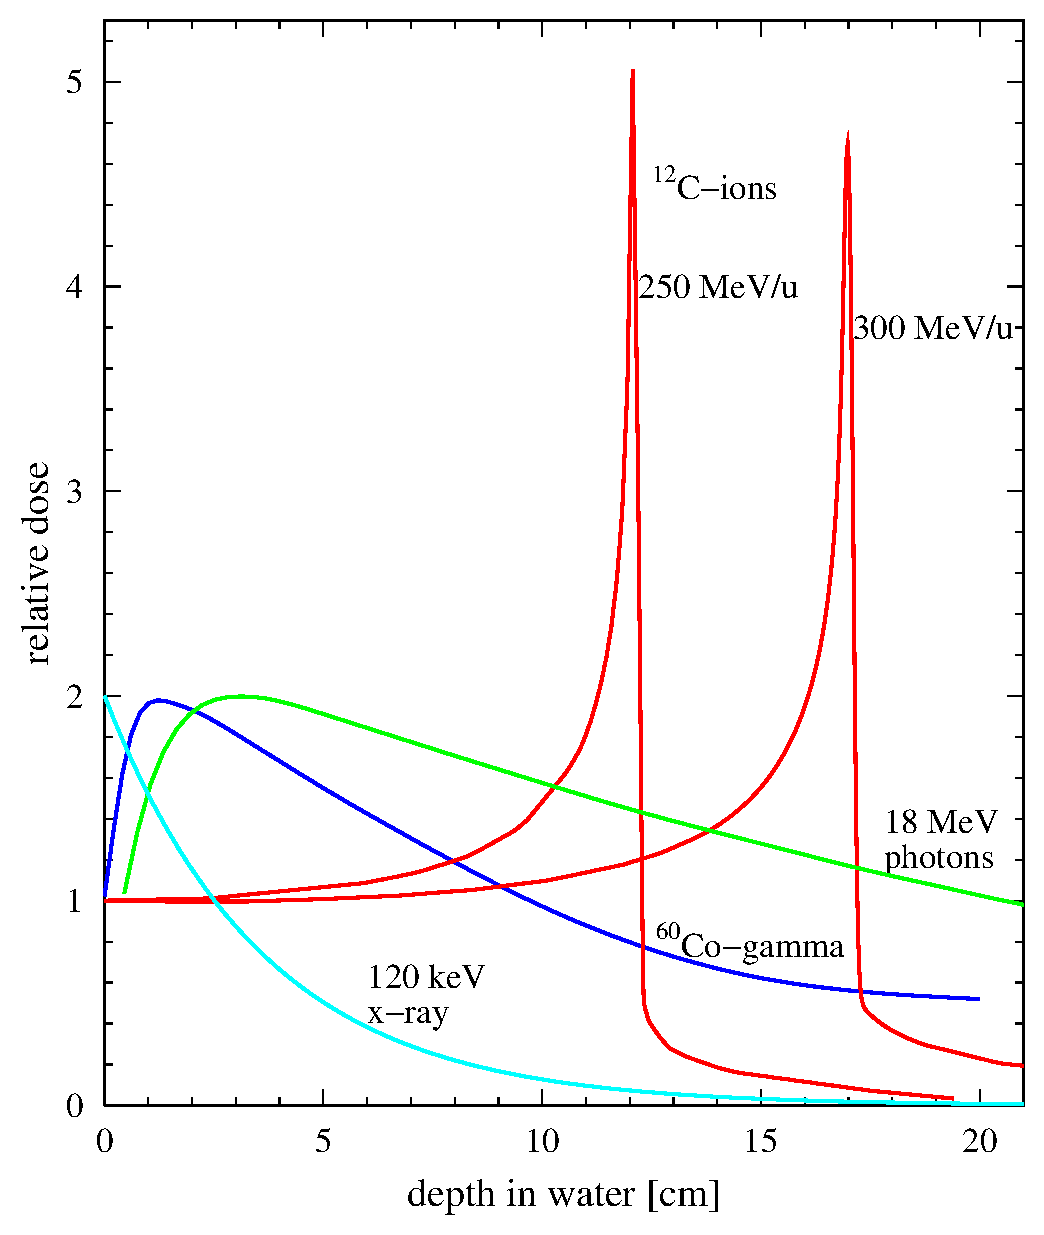
\includegraphics[scale=1]{depthdose.eps}
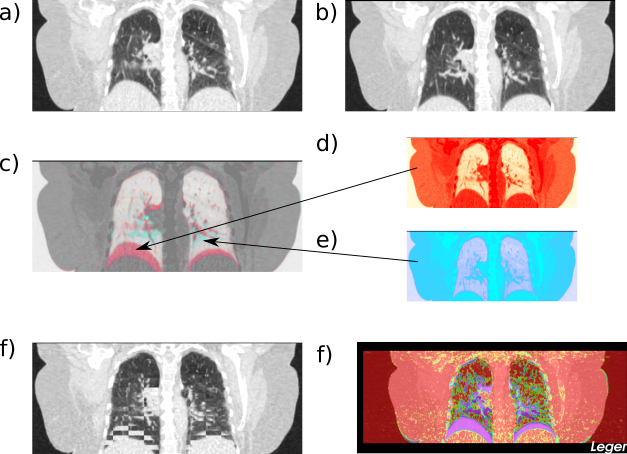
\includegraphics[width=0.9\textwidth]{./Images/dirqa.png}
\caption{Different registration quality image checks of reference (a) and warped image (b). While there is not trivial to spot differences when images are side by side, the task is much easier if they are overlayed in
opposite colors (c), as explained in Sec.~\ref{Sec:FalseColor}. False color is made by using red color code on reference (d) and blue on warped image (e). Arrows point to areas in false color where there are differences between
the two images. The differences are also clearly see on checkerboard image (f) and are stressed on root mean square \textbf{?} image (g).}
\label{Imagedirqa}
\end{center}
\end{figure}

\subsubsection{Output file}

With all different features to validate DIR it can be time consuming to go through them all. A special option was created to automatically go through all different validation steps. Furthermore it can also run through different phases, if there are more phases (i.e. in 4DCT). All produced data from DIR validation is stored on disk and can be reexamined by user upon request. Furthermore, images are created and data is summed up and displayed in a separate file. Users can then preview file for first validation of DIR and then open necessary files, if required.

\subsection{Contour visualization}
\label{Contour}

TRiP4D (see Section \textbf{REF}) introduced volume datasets for contour representation \cite{Richter2012}. It enabled necessary tasks for 4D calculations, such as the storing contour in different 4D states, contour propagation, etc. However, there was a lack of a proper visualization tool. In order to provide a contour visualization tool, a Slicer module was created. 

Contours are saved as volumetric boolean masks. A single bit per ROI contour representation marks each voxel inside volume dataset \cite{Richter2012}. To properly display contour, first a whole volume dataset was imported in Slicer. User selects which motion state he would like to inspect. The corresponding bit is then selected on the imported volume dataset. Lastly the contour is converted into 3D model shape. 

\subsection{Motion estimation and ITV creation}

ITV is often created by an eye investigation of all 4DCT phases, where the extent of motion is estimated. Automatic creation of ITV is scarce in commercial system, since it requires DIR on all 4DCT phases. A Slicer module was created to assist with the motion estimation and automatic ITV creation using DIR. 

Module is able to estimate and display motion of a user selected contour in three axis (left-right, anterior-posterior, superior-inferior) based on DIR vector fields. Module also performs DIR on 4DCT with patient hierarchy, if it has not been done yet.

Beside motion estimation, module can also propagate selected contour (usually CTV) and propagate it to all 4DCT and make a convolution of all propagated contours, resulting in automatic generated ITV.

\subsubsection{Generation of mid-ventilation phase}






\section{Verification}
\label{Verification}
\section{Summary and Discussion}


\bibliographystyle{apalike}
\bibliography{../ref.bib}{}
% \bibliographystyle{plain}

\end{document}
